\documentclass[11pt]{article}
\usepackage[utf8]{inputenc}
\usepackage[a4paper, total={6.5in, 9in}]{geometry}

\title{SPROJ}
\author{Derek Low}
\date{2017-2018}

\usepackage{natbib}
\usepackage{graphicx}
\usepackage{upgreek}
\usepackage{amsmath}
\usepackage{float}
\usepackage[font=scriptsize,labelfont=bf]{caption}
\captionsetup{justification   = raggedright,
              singlelinecheck = false}
\renewcommand{\baselinestretch}{1.6}

\begin{document}

\maketitle

\section{Introduction}

\subsection{The Neuron}
Neurons are fundamental units of human cognition, and allow for a large range of activities such as movement, speech, decision making, and learning among many other functions in the human body. The interactions between neurons throughout the human body is studied and understood, to a limited extent, at microscopic levels; such studies may concern the signal propagation along neurons in the hippocampus (Hoffman et al., 1997), or the dynamics of the synapse, the structure of connection between neurons, and implications of changes to those dynamics (Haydon, 2001; Terry et al., 1991). Additionally, interactions between neurons are studied at macroscopic levels, where certain areas of the brain are responsible for certain functions of the nervous system, such as the relationship between the prefrontal cortex and human capabilities of cognitive control and activity (Miller and Cohen, 2001), or sensorimotor cortex activity and the resulting motor imagery and action (Porro et al., 1996). However, the precise connectivity patterns of neurons, and the relationship between this organization and its possible functions, are not fully understood. Analysis of the patterns of connections in populations of neurons indicate that these cells are characterized by certain network properties, and are not completely random. Understandings of these connections may provide insight to the function and activity of these populations of neurons, as well as divulging further characteristics of the neuron populations from a graphical point of view, such as clustering coefficients and distances (Sporns et al., 2004).\par

The activities of neurons are partially mediated by the electrical potential between the neuron and its surrounding environment, known as the membrane potential; changes in concentrations of ions distributed in varying concentrations throughout the nervous system drive neuron activity by changing this membrane potential. In a state of low activity, this membrane defaults to a polarized state of negative electrical potential, referred to as the resting membrane potential (Purves et al., 2004). Communication between neurons occur at the synapse, a location of connection between two neurons, via synaptic potential, and is intiated by the release of neurotransmitters from the presynaptic neuron to receptors in the postsynaptic neuron. Synaptic potentials are either excitatory, increasing the membrane potential of the neuron towards positive values (depolarization), or inhibitory, reducing potential towards negative values (hyperpolarization). The resulting depolarization due to the excitatory post-synaptic potentials (EPSPs) increases the membrane potential towards higher positive values, until a particular threshold is reached. Once this threshold potential is reached, an action potential is generated, and propagates along the neuron until it reaches another synapse, at which point the cycle of neurotransmitter release, synaptic potential, and action potential propagation cycle may be repeated.\par

The earliest and most influential studies concerning the effects of ions in neurons were conducted by Hodgkin, Huxley, and Katz nearly 70 years ago, and clearly indicated the impact of sodium concentration on the activity of neurons; giant squid axons in lower sodium environments demonstrated a lower resting potential, as well as a weaker and delayed action potential (Hodgkin and Katz, 1949). Potassium concentration demonstrates a similar impact to the membrane potential, with a reduced concentration resulting in higher resting and action potentials and a shallower repolarization of the membrane (Hodgkin and Katz, 1949). Membrane potential is quantified by the polarity of these ionic molecules, and their respective concentrations on each side of the membrane, or the difference between the intracellular and extracellular concentrations of the ion.\par

The propagation of action potentials involves constant changes to the electrochemical gradients of the neurons by the opening and closing of ion channels in the membrane. The changes in channel structure mediate the process of depolarization. The mechanisms governing and driving membrane potentials towards depolarization and repolarization are the voltage-gated ion channels, a family of channels that include the sodium (Na\textsuperscript{+}), potassium (K\textsuperscript{+}) and calcium (Ca\textsuperscript{2+}) channels. However, while these channels serve similar purposes of allowing passage to certain ions and restricting passage to other ions, the time of activation of each type of channel demonstrated their distinct impacts on propagation. Early researchers discovered and verified the significance of sodium on the depolarization of the nueron and the initiation of an action potential, suggesting the entry of sodium to be the carrier of voltage into the neuron (Hodgkin and Katz, 1949; Hodgkin and Huxley, 1952). Furthermore, the resulting repolarization and hyperpolarization stages preceding the return to resting membrane potential result from the efflux of potassium; this efflux is a delayed response to the initiation of the action potential, indicating a delayed opening of potassium channels following the opening of sodium channels (Hodgkin and Huxley, 1952).

%STUFF THAT I MAY OR MAY NOT INCLUDE:
%In particular, Na\textsuperscript{+} channels contain a segment, referred to as the S4 segment, dedicated to sensing intracellular voltage changes (Armstrong and Hille, 1998).  These changes occur through a variety of manners; in the most general sense, systems with differences in concentrations, whether these systems are concerned with ionic concentrations or involve thermal dynamics, tend to move towards a state of equilibrium, where the concentration is diffused across the entirety of the space available. Molecules in and between neurons are no exception to this tendency, and move toward electrochemical equilibrium across the membrane.\par

\subsection{Network Neuroscience}

Studies have noted the possible relationshps between the connectivity of neurons and their developmental and functional consequences. Network science provides a framework through which populations of neurons may be analyzed for their structural and functional connectivities by expanding and formalizing the terminologies and definitions for the purposes of neuronal network analysis. Cliques, or all-to-all connected networks, of neuronal populations have been studied as a method of relating structural and functional connectivities of neuronal populations; in the context of neuronal networks, cliques are observed under a specific definition, the directed clique. Where cliques are bidirectional, allowing a single connection for both information transfer from a source neuron to a target neuron and information transfer in the inverse direction, directed cliques do not allow for bidirectional information transfer. (Reimann et al., 2017). Thus, for a given connection from a source neuron to a target neuron, there is no direct connection from the target neuron to the source neuron, though there may be an intermediary neuron allowing for a connection in the inverse direction. The small world characteristic is another such definition originating from network science and applied in analysis of neuron populations, where the small world network is a network with a short average path length, indicating a large number of paths, and a high degree of local clustering, the tendency of nodes in a graph to cluster together (Sporns et al., 2004).\par

Further analysis of these patterns of connectivity, or microcircuitry, of neurons in regions of the brain indicate the possibility of the scale-free nature of microcircuits. In cases of such networks, the degree distribution, defined as the distribution of number of connections to each node in a give network, follows a power-law, where the majority of nodes in the network have a high number of connections, and a fraction of the population with a comparatively low number of connections (Sporns et al., 2004, Tetzlaff et al., 2010, Massobrio et al., 2015). This power-law distribution is also observed in the 
%here, start relating to more neurobio things, such as what Arseny mentioned (stuff you have written in your notebook)

%perhaps I should add a formal definition of clustering coefficient here.


The relationship between functionality and connectivity has been demonstrated in further additional contexts, such as in motor neurons of human patients by relating the movement of fingers on each hand to the flutuations in signal intenstiy of the sensorimotor cortex during echo-planar functional magnetic resonance imaging (fMRI)(Biswal et al., 1995). Additionally, between two related, yet distinct, activities, the functional connectivity of neurons can overlap; such is the case in the instance of motor imagery, or the mental performance of certain motor acts not accompanied by physical performance of these acts, and the accompanying physical performance of the same motor acts (Porro et al., 1996). The hippocampus of the human brain demonstrates a similar relationship of functional connectivity with particular activities; young adults display higher levels of activity in the ventral prefrontal and extrastriate regions of the cortex correlated with higher levels of hippocampus activity during  encoding of words and pictures of objects. In contrast, older adults display higher levels of activity in the dorsolateral prefrontal and parietal regions of the cortex with comparable levels of activity in the hippocampus to younger adults during similar trials (Grady et al., 2003). The higher activity in particular regions implies different manners by which adults of differing ages process information concerning similar tasks, where hippocampus and brain activity are related to better recognition in younger adults, and improved memory performance in older adults. These findings indicate a shift in explicit connectivity between portions of the brain, and changes to functional connectivity related to human aging (Grady et al., 2003).\par

The configuration of neurons and network properties of these particular networks are significant not only to the function of the network, but to developmental implications as well. The discussion of the development of neurons typically relates to the discussion of network dynamics in networks of neurons during stages of growth, or to the adaptability and learning capabilities of these neurons. Concerning the former case, studies discuss the continuous process of reconfiguration during stages of development.



\subsection{Representing Networks of Neurons}
Deriving the organization of neurons in networks is difficult at lower populations of neurons, and the difficulty increases significantly as the population of neurons increases. The organization of neurons can be represented as a matrix, typically referred to as an adjacency or weight matrix; whether the matrix is an adjacency or weight matrix depends on how these connections between neurons are represented, and what information is useful and preserved. Weight matrices assign values based on the strength of connections between neurons, and whether the source neuron is an excitatory or inhibitory neuron, while adjacency matrices are representative of whether or not there is a connection, and ignores the strength of these connections. For example, the following matrix describes connections between a population of three neurons:\par
\begin{figure}[H]
\begin{center}
\begin{tabular}{ |p{3cm}|p{3cm}|p{3cm}|p{3cm}|  }
 \multicolumn{4}{}{}\\
 \hline
  & Neuron 1 & Neuron 2 & Neuron 3\\
 \hline
 Neuron 1 & 0 & 1 & 1\\
 Neuron 2 & 0 & 0 & 0\\
 Neuron 3 & 1 & 1 & 0\\
 \hline
\end{tabular}
\end{center}
\caption{Sample Adjacency Matrix of a Population, Size 3. Diagonal indices represent self-connections. Labels along the columns represent the target, and labels along the rows represent the source e.g. the connection at Row 3, Column 2 (value of 1) is a connection from the pre-synaptic Neuron 3 to the post-synaptic Neuron 2. Note the lack of the inverse connection from Neuron 2 to Neuron 3 (value of 0).}
\end{figure}

Matrices such as the one above describe the connections between different neurons in an observed population, with observed being an important keyword; these neurons could have incoming connections from sources outside of the observed population, depending on the context of the observations. One standard feature of network matrices is the zero value along the diagonal, representative of a lack of a connection from a neuron to itself. In the example above, there is a directional connection between the outward axonal connection of Neuron 3 and the incoming dendritic connection of Neuron 1; therefore, assuming a positive value to represent an excitatory connection, spikes in Neuron 3 result in a voltage increase of Neuron 1. By this method of representation, the matrix can describe the relative strength and nature of all connections between neurons in the observed population.\par

Why is it important to characterize networks of neurons? Currently, our methods of studying neurons and brain activity relies on techniques that observe activity at macroscopic (e.g. fMRI, PET, CAT, calcium imaging) or microscopic scales (e.g. electrodes and membrane potentials, patch clamp). However, there is no method of accurately imaging and representing larger networks of neurons in areas of the brain, or outgoing pathways from the brain. While machine learning algorithms may not provide exact mappings of networks, implementation of these algorithms is an opportunity to generate hypotheses.\par

\subsection{Calcium Imaging}
A commonly employed method of recording activity of neurons is calcium imaging. Neuron activity . At every spiking event, these ions travel through the cell membrane of each neuron by movement through voltage-dependent ion channels, which are functionally altered by the voltage changes that occur in neurons.\par

The versatility and presence of calcium in neurons can be described by the large variety of neuronal processes related to it. Calcium performs several major roles in the function and management of biological cells; most notably, in the presynaptic neuron, an influx of calcium into the neuron triggers the release of neurotransmitter to the synapse via exocytosis (Katz and Miledi, 1967). Furthermore, presynaptically, residual calcium results in neural facilitation, a period in which a successive depolarization of the presynaptic neuron, following the first depolarization event and release of neurotransmitter, raises the likelihood of neurotransmitter release (Katz and Miledi, 1967; Zucker, 1999). Postsynaptically, calcium is responsible for activating the synaptic plasticity cascade. These changes to the synapse, functionally initiated by interactions between calcium and the N-methyl-D-aspartate receptor (NMDA) and $\alpha$-amino-3-hydroxy-5-methyl-4-isoxazolepropionic acid receptor (AMPA), result in changes to the sensitivity and, by extension, the interactions between the pre- and postsynaptic neurons (Zucker, 1999). The changes enhance or diminish the strength of the connection (potentiation and depression), in various temporal manners (short and long-term). For example, in the case of long-term potentiation (LTP), the influx of calcium into the postsynaptic neuron, and the resulting depolarization, result in the unblocking of the NMDA receptors, allowing for a further influx of calcium into the postsynaptic neuron and inducing LTP (Zucker 1999).Functions of calcium extend further than synaptic activity, and the ion is additionally responsible for biological functions such as cell apoptosis (Orrenius et al., 2003). Therefore, the abundance and utility of calcium, and the deeply integral relationship between calcium and neuron activity, suggest it to be a strong candidate for the purpose of imaging populations of neurons.\par

\subsubsection{Calcium Indicators}
As mentioned, calcium activity is dependent on the voltage changes of neurons and the responses of voltage-gated channels to voltage changes, and concentration is higher extracellularly until spike time. Therefore, introducing into the neurons an indicator that fluoresces when bound to calcium allows recording of calcium concentration and activity. Among the first discovered and applied calcium indicators is the protein aequorin (Shimomura et al., 1962), where the binding of the calcium to the three binding sites located on the protein results in photon emission (Grienberger and Konnerth, 2012). The necessity of the three calcium molecules, in combination with a controlled amount of indicator injected into these neurons, allows for a controlled fluorescence method that is directly related to the calcium concentration within the cell. However, the particular drawbacks of aequorin, such as a low protein stability and a relatively low fluorescence rate with regards to the amount of decomposition in the concentration of the protein, result in development of several superior and modern alternatives (Grienberger and Konnerth, 2012).\par

Modern calcium indicators are typically categorized as high-affinity or low-affinity, where high-affinity indicates the most commonly used indicators with wide varieties of application. One such high-affinity calcium indicator is fura-2 (Grynkiewicz et al., 1985); this indicator operates by excitation with ultraviolet light, resulting in a fluorescence shift of the indicator; the fluorescence level changes when the molecule is bound to calcium, a property referred to as ratiometric, dual-wavelength, or dual-excitation (Grienberger and Konnerth, 2012). This particular indicator is applied to a variety of microscopy methods, including two-photon microscopy (discussed below), requiring slight modification by inclusion of green fluorescent protein (GFP) in the latter case (Grinberger and Konnerth, 2012). 

\subsubsection{Microscopy}
The second component is the imaging, recording, and approximation of recorded data as a measurement of brain activity. There are several technologies employed in the recording of calcium indicator fluorescence; the technique used widely depends on the subject being recorded and quality of the imaging required. However, an equally wide range of techniques are available, and have particular benefits and drawbacks relating to the method and observed sample.\par

All microcopy techniques result in the photobleaching and phototoxicity of the observed specimens, resulting in photodamage (Svodoba et al., 2006). Another restricting factor in microscopy is photon scattering, a process in which a photon is absorbed by a molecule and re-emitted in a distinctly random direction, resulting in the blurring of the resulting microscopy image (Ntziachristos, 2010). Therefore, one aim relevant to employed microscopy techniques is the highest accumulation of imaging data with the lowest possible amount of photodamage to the observed specimen, and lowest photon scattering for image accuracy and clarity. Prior to the development of two photon microscopy in the 1990's (Denk et al., 1990), most microscopy methods used, such as confocal and wide-field fluorescence microscopy, suffered from the major drawback of having low tissue penetration depth due to photon scattering and, in the case of confocal microscopy, tissue degredation (Svodoba et al., 2006).

\subsection{Current Approaches to Reconstruction}
Several different frameworks of reconstruction have been offered to tackle the problem of inferring connectivity of neurons. While these reconstruction methods use different methods for evaluating activity and connectivity, they are typically applied to simulated neuron populations, where the ground truth of the activity is known, allowing evaluation on the accuracy of the model.\par

\subsubsection{Cross-Correlation}


\subsubsection{Granger Causailty}
Zhou et al., 2014 uses Granger Causality as the primary method of inferring connectivity of conductance-based integrate-and-fire neuron models; the analysis method states that if the variance in prediction error for a particular time series is reduced by incorporating knowledge of another time series, then the second time series has some causal effect on the first time series. In other words, if incorporating information about event X allows prediction of event Y beyond prediction concerning event Y without any additional information, then event X and event Y are causally related.  In brief, the researchers demonstrate that using Granger Causality allows the construction of a causality matrix, which can then be mapped to the structural connectivity matrix of the population and be observed for relationships between the activity and structure of the network.\par

\subsubsection{Transfer Entropy}
Stetter et al., 2012, incorporates information theory as a reconstruction method from calcium imaging data. This particular method of reconstruction focused on in vitro calcium imaging fluorescence levels, with a slightly variant version of the Generalized Transfer Entropy formula:

$$TE_{Y->X}(\hat{g}) = \sum{P(x_{n+1}, x_x^k,y_{n+1}^k|g_{n+1}<\hat{g}}) log \frac{P(x_{n+1}|x_n,y_{n+1}^k,g_{n+1}<\hat{g}}{P(x_{n+1}|x_n^k,g_{n+1}<\hat{g}}$$

The major difference between the Generalized Transfer Entropy formula and the presented formula is the presence of $\hat{g}$, a predefined threshold of fluorescence, where $g_t$ is the average fluorescence of the network at a particular time $t$.\par

The researchers use Transfer Entropy to evaluate the information transfer, where information transfer can be understood as how likely the activity of neuron Y indicates the activity in neuron X, between all possible directed pairs of neurons in the network. Afterwards, the researchers use a threshold Transfer Entropy to prune the the connections with the lowest values of information transfer, and reconstruct the network based on the remaining neurons, finding Transfer Entropy to reconstruct network properties more accurately than previous reconstruction methods, and at varying levels of visual noise in the data, or light scattering.\par

\subsection{The Relevance of Advances in Machine Learning}
The story concerning the invention and development of machine learning is one of constant juxtapositions with human intelligence. For example, the perhaps one of the most famous early experiments in artificial intelligence research is the Turing Test. The Turing Test, devised by Alan Turing, was originally named "The Imitation Game" by Turing in the 1950 paper "Computing Machinery and Intelligence". The experiment was devised with the proposed definition of artificial intelligence as the ability of a machine to replace a human counterpart in repeated rounds of questioning and answering; in other words, is the machine capable of imitating a human to the extent that participants are fooled by its answers? The performance evaluation of the machine is defined as a comparison with human intelligence, and as an antagonist to human interaction. Naturally, in the consistent comparison with human intelligence as benchmarks for machine intelligence, artificial intelligence research eventually developed methods of machine learning loosely based in the fundamental biological unit of human intelligence: the neuron.\par

As discussed previously, neurons are the fundamental units that allow what we understand to be human intelligence. As discussed by Steels in the paper "Fifty Years of AI: From Symbols to Embodiment", the field transitioned through several methods and approaches to AI before arriving at the neural network in the 1980s (Steels, 2007). These neural networks were developed with the intent to model the biological mechanisms of the human brain as closely as possible, primarily the neurons, which the nervous system is composed of. Even in the short history of neural networks, the method has transitioned through varying degrees of discovery and standardization concerning their usage and applicability.\par

\subsubsection{Supervised and Unsupervised Learning}
While the studies of machine learning have developed a variety of methods to encompass an ever-growing scope of questions to answer, the methods and questions fall into one of two categorizations: supervised and unsupervised learning. Supervised learning methods rely on the "completeness" of a data set, in which all inputs have correspondingly labelled outputs. Therefore, the output of a supervised learning algorithm is similar in type to the actual outputs $Y$ presented in the training data set for every $X$; in other words, there is a corresponding dependent output on the independent input. The natures of the inputs and outputs are variable, and need not necessarily be of the same type; for example, an input of an image can result in a categorization of the image contents, such as "dog" or "human". They can also be numerical, such as a prediction of grade based on the input amount of time studying (Hastie et al., 2009). In these two examples, the prior is an instance of qualitative, or categorical, prediction, while the latter is a quantitative, or regression, prediction.\par

Unsupervised learning differs in that there is no input-output; while there are $X$ labels, there are no corresponding $Y$ labels. Some neural networks fall under this classification of algorithms; for example, Pandarinath et al. 2017, introduces an algorithm that uses sequential auto-encoders to infer underlying patterns of spike trains. Auto-encoders are one example of unsupervised learning, where the network receives an input $X$, attempts to represent underlying patterns in the data, and recreate the input as the network's output. 

\subsubsection{Artificial Neural Networks}
As discussed, neural networks are based on the morphology of human brains, and the neurons that the brain is composed of. These networks are composed of some number of nodes, or neurons, that are connected to each other in some fashion, depending on the task the particular network is designed for. These nodes are typically categorized into one of three layers: input, hidden, and output layers. Neurons of the input layer have no predecessor neurons, and neurons of the output layers have no following neurons; instead the the input neurons receive input information of a particular data set, and the output neurons displayed the expected outputs based on the inputs to the network and the corresponding hidden layers.\par

The general theory behind Artificial Neural Networks can be described as a metaphor to learning; just students prepare for exams by thoroughly studying and applying knowledge repeatedly prior to the exam, neural networks typically train on large data sets by taking an input $X$, and producing some inferred output $Y$, then comparing to the actual output that is provided by the corresponding input in the data set to calculate the error between the prediction and the true output reflected in the data set. This data set is referred to as the "training set", on which the neural network  metaphorically prepares for the exam. The goal of this training is to adapt the system to handle situations that are not contained within the training set, and predict these outputs with accuracy based on the training information provided to the network (Werbos, 1990).\par

\subsubsection{Hidden Layers}

\subsubsection{Backpropagation}
Backpropagation is one of the most recognized techniques in the study of neural networks. Developed by Paul Werbos in the 1970's, backpropagation is the primarily used method of learning in neural networks. The method is so named because the updating of weights at every layer begins at the final layer, and propagates backwards to every node and weight until all weights of all nodes in each layer have been updated to correct for the calculated error in the network.

\subsubsection{Gradient Descent}


\subsection{NEST: Generating Training Data}
There are several reasons for generating simulated calcium imaging data for the purposes of network reconstruction. First, generation of simulated calcium imaging data allows for benchmarking of the reconstruction methods employed. In typical calcium imaging data, the ground truth is not known, resulting in a lack of comparison between the reconstructed network and the network targeted for reconstruction. By generating simulated networks and recreating calcium imaging data, we ensure access to the ground truth for comparison with the model. Simulation of training data also permits programming of particular characteristics to the network, and observing the changes of this reconstruction in both the simulated data and the reconstruction of these networks.\par
Machine learning methods are typically trained on some prior data set; simulation of calcium imaging data provides a easy method of accessing data for training and testing the machine learning based model, due to unconstrained and unrestricted access to training data, before allowing the model to analyze recorded data that would be ideally used as testing data. Additionally, including a training set ensures that the algorithm is able to remain “generalized”; that is, the algorithm does not learn to represent that single data set exceptionally well, and fail when a different pattern is presented to the algorithm.\par
The simulations presented here are performed in NEST simulator, a tool maintained by the NEST initiative. The NEST simulator was selected for the purpose of simulations that maintain biological realism and complexity, with emphasis on simulation of large neuronal networks. The advantage NEST has over other simulators is the capability to simulate large networks with varying facets, such as synapse and neuron types, while retaining accurate representation of the individual neurons.\par

\section{Methods}

\begin{figure}[H]
\centering
	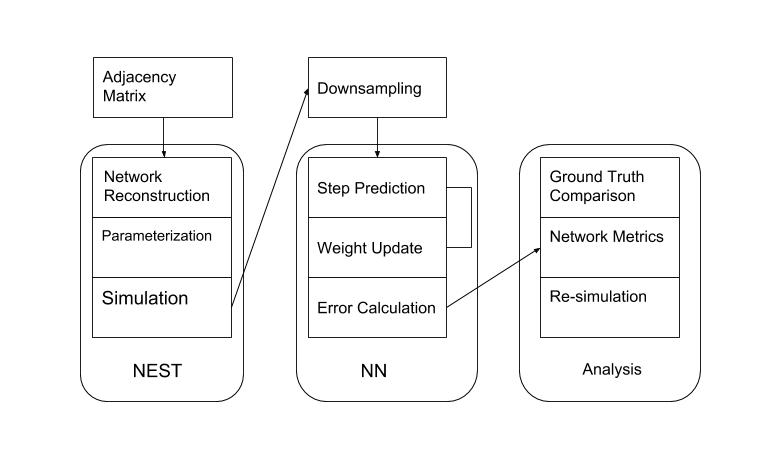
\includegraphics[scale=0.4]{./Figures/SPROJModel.jpg}
	\caption{Experimental Pipeline. We start with a pre-generated adjacency matrix detailing the connections of a population of neurons, and pass it to the NEST simulator program. The NEST simulator reconstructs the network defined by the matrix; at this stage, poisson noise is added to the population via a connection from a 'noise generator' NEST object to all neurons in the population. The simulation is then run for 10000 timesteps (milliseconds), and the generated data is output as a spiketime matrix of n x t dimensionality, n = population size and t = timesteps. The output is then downsampled to reflect realistic calcium imaging frame duration of 10 ms, reducing the data set to t = timesteps/10.\\
The downsampled data is then trained in the neural network via comparison of previous timestep to next timestep, using mean squared error and backpropagation. After some predetermined iteration value or conditional is reached (such as error convergence), the network outputs the resulting weight matrix, which can then be analyzed with respect to the ground truth adjacency matrix passed in the first stage of the pipeline.}
\end{figure}

\subsection{Simulation of Neurons for Spike Train Generation}
The NEST simulator is used for the purposes of generating spike train data. NEST Izhikevich neurons are used as the model neurons, due to the increased complexity over leaky integrate-and-fire neurons, and the reduced computational complexity over models of significantly more numerous compartment models, such as the Hodgkin-Huxley models (Brette, 2015). NEST implementation dynamics of Izchikevich neurons are provided by the following :

$$dv/dt=0.04v^2+5v+140-u+I$$
$$du/dt=a(bv-u)$$
\smallskip

{\centering
if $v >= V_{th}:\{$\\
$v = c$\\
$u = u + d\}$\par
}
where $v$ represents the membrane potential of the neuron and $u$ the membrane recovery variable. The membrane recovery variable captures the responses of $K^{+}$ and $Na^{+}$, and is a source of negative feedback to $v$. Coefficients for change in membrane potential, are based on scale, with membrane potential at $mV$ and time as ms, as are $a$ and $b$. $I$ is the input current to the neuron, and $c$ and $d$ are the post-spike reset values of the neuron (Kunkel et al., 2017, Izhikevich et al., 2004). 

To simulate a population of neurons with $n$ population size over $t$ time, a file containing an $n x n$ adjacency matrix is provided to the simulation program, which then creates a NEST neuron population with the exact number of neurons and connections between the neurons in the population, using the corresponding weight of the connection stored in the adjacency matrix. Interactions with neurons in NEST must be achieved through the creation of new node objects, made to represent and achieve the results of physical instruments and devices; therefore, we create a poisson generator node to add noise to the population, and connect a spike detector node to record all spikes in the population during simulation. The population is then recorded over 10000 simulation steps, or 10000 ms. The corresposnding output of the simulation is converted to a matrix of n x t dimensionality.\par
\begin{figure}[H]
\centering
	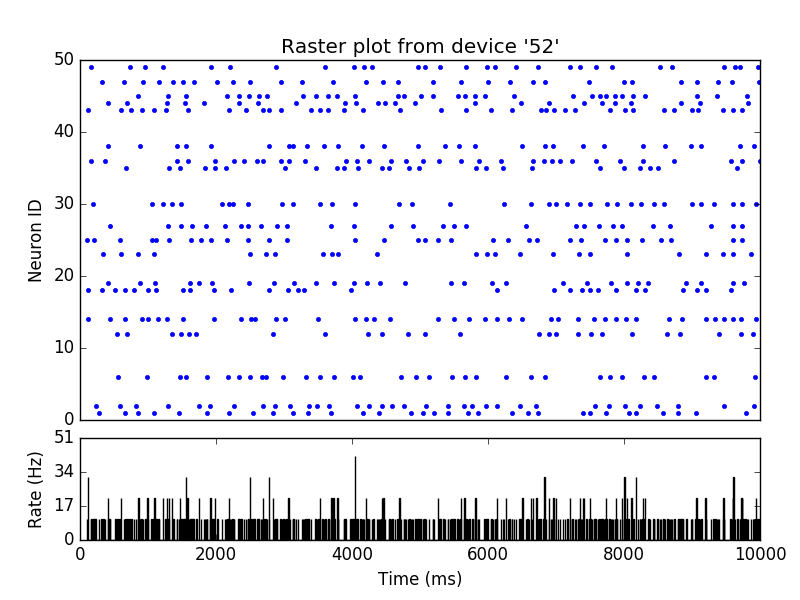
\includegraphics[scale=0.5]{./Figures/figure_1.png} 
	\caption{Raster Plot via NEST Simulator. The plot is generated by simulating a population of 50 neurons over 10000 time steps (ms), and graphically represents two distinct arrays output by the simulation: one array consisting of neuron IDs in the population, and another array with the corresponding spike times of the spiking neurons stored in the indices of the former array. The NEST simulator connects each neuron based on the input adjacency matrix and attaches additional noise and spike detection objects to every neuron in the population. Device 52 is the NEST spike detection object; all neurons are connected by the NEST simulation program for the purposes of spike detection. Device 51 is the noise generator object, and Devices 1-50 are the neurons in the population. }
\end{figure}

\subsection{PageRank}
The PageRank-based algorithm takes a weighted adjacency matrix as an input; a non-weighted adjacency matrix would result in no change in the PageRanks of each neuron, and no change in the resulting adjacency matrix. The PageRank for each neuron is then calculated based on the following formula:

$$PR_i = (1-d)+d(\sum(\frac{PR_j}{C} * W_ij))$$

Where PR is the PageRank of neuron $i$, $d$ is the standard damping factor of 0.8, $PR_j$ is the PageRank of incoming neuron j, and $W_{ji}$ is the weight of the connection from neuron j to i. The summation calculates for all incoming connections to neuron i. The formula is recalculated until convergence, where the PageRanks no longer change, at which point the weights are updated such that the weight of each connection is multiplied by the PageRank of the source of the connection. The network is then pruned by comparing the weights between neuron i and j, or Wij and Wji, and the the lower value is reduced to 0, while the higher value is set to 1, preserving the higher connection. The process is then repeated, using the new weights, for an arbitrary number of times.\par
\section{Results}

\section{Conclusion}

\section{Works Cited}
\bibliographystyle{plain}
\bibliography{references}
\begin{enumerate}
\item Alberts B, Johnson A, Lewis J, et al. Molecular Biology of the Cell. 4th edition. New York: Garland Science; 2002. Ion Channels and the Electrical Properties of Membranes. Available from: https://www.ncbi.nlm.nih.gov/books/NBK26910/
\item Armstrong, C. M., \& Hille, B. (1998). Voltage-Gated Ion Channels Review and Electrical Excitability Early Biophysics and Voltage Clamp Revealed Voltage-Gated Membrane Permeabilities The period from 1939 to 1952 was a heroic time in the. Neuron, 20, 371–380.\\ https://doi.org/10.1016/S0896-6273(00)80981-2
\item Biswal, B., Yetkin, F. Z., Haughton, V. M., \& Hyde, J. S. (1995). Functional Connectivity in the Motor Cortex of Resting. Magnetic Resonance in Medicine, 34(4), 537–541.
\item Brette, R. (2015). What Is the Most Realistic Single-Compartment Model of Spike Initiation? PLoS Computational Biology. https://doi.org/10.1371/journal.pcbi.1004114
\item Brette R, Rudolph M, Carnevale T, et al. Simulation of networks of spiking neurons: A review of tools and strategies. Journal of computational neuroscience. 2007;23(3):349-398. doi:10.1007/s10827-007-0038-6.
\item Denk, W., Strickler, J. H., \& Webb, W. W. (1990). Two-Photon Laser Scanning Fluorescence Microscopy. Science, 248(4951), 73–76.
\item Garofalo, M., Nieus, T., Massobrio, P., \& Martinoia, S. (2009). Evaluation of the Performance of Information Theory- Based Methods and Cross-Correlation to Estimate the Functional Connectivity in Cortical Networks. PLoS ONE, 4(8).\\https://doi.org/10.1371/journal.pone.0006482
\item Grady, C. L., McIntosh, A. R., \& Craik, F. I. M. (2003). Age-related differences in the functional connectivity of the hippocampus during memory encoding. Hippocampus, 13(5), 572–586. https://doi.org/10.1002/hipo.10114
\item Grynkiewicz, G., Poenie, M., and Tsien, R.Y. (1985). A new generation of Ca 2+ indicators with greatly improved fluorescence properties. J. Biol. Chem.260 , 3440–3450
\item Hastie T., Tibshirani R., Friedman J. (2009) Overview of Supervised Learning. In: The Elements of Statistical Learning. Springer Series in Statistics. Springer, New York, NY
\item Haydon, P. G. (2001). GLIA : LISTENING AND TALKING TO THE SYNAPSE. Nature Reviews Neuroscience, 2(March), 186–193.
\item Hecht-Nielsen, R. (1989). Theory of the Backpropagation Neural Network. Proceedings Of The International Joint Conference On Neural Networks, 1, 593–605.\\https://doi.org/10.1109/IJCNN.1989.118638
\item Hodgkin, A. L., \& Kats, B. (1949). The Effect of Sodium Ions on the Electrical Activity of the Giant Axon of the Squid. The Journal Of Physiology, 108(1), 37–77.
\item Hoffman, D. A., Magee, J. C., Colbert, C. M., \& Johnston, D. (1997). K + channel regulation of signal propagation in dendrites of hippocampal pyramidal neurons. Nature, 387(June), 869–876.
\item Izhikevich, E. M. (2004). Which model to use for cortical spiking neurons? IEEE Transactions on Neural Networks. https://doi.org/10.1109/TNN.2004.832719
\item Katz, B., \& Miledi, R. (1967). A Study of Synaptic Transmission in the Absence of Nerve Impulses. Department of Biophysics, University College London, 407–436.
\item Katz, B., \& Miledi, R. (1968). The role of calcium in neuromuscular facilitation. Journal of Physiology, 195, 481–492. https://doi.org/10.1111/j.1365-3040.1992.tb01004.x
\item Kunkel, Susanne, Morrison, Abigail, Weidel, Philipp, Eppler, Jochen Martin, Sinha, Ankur, Schenck, Wolfram, … Plesser, Hans Ekkehard. (2017, March 1). NEST 2.12.0. Zenodo. http://doi.org/10.5281/zenodo.259534
\item Marblestone, A., Wayne, G., \& Kording, K. (2016). Towards an integration of deep learning and neuroscience. https://doi.org/10.3389/fncom.2016.00094
\item Massobrio, P., Pasquale, V., \& Martinoia, S. (2015). Self-organized criticality in cortical assemblies occurs in concurrent scale-free and small-world networks. Nature Publishing Group, (October 2014), 1–16. https://doi.org/10.1038/srep10578
\item McCulloch, W. S., \& Pitts, W. H. (1943). A Logical Calculus of the Ideas Immanent In Nervous Activity. Bulletin of Mathematical Biophysics, 5, 115–133.
\item Miller, E. K., \& Cohen, J. D. (2001). An Integrative Theory of Prefrontal Cortex Function. Annual Review of Neuroscience, 24, 167–202.
\item Minshew, N. J., \& Williams, D. L. (2007). The New Neurobiology of Autism: Cortex, Connectivity, and Neuronal Organization. Archives of Neurology, 64(7), 945–950.
\item Mitchell, M. (1996). An Introduction to Genetic Algorithms (5th ed.). Cambridge, MA.: MIT Press.
\item Ntziachristos, V. (2010). Going deeper than microscopy : the optical imaging frontier in biology. Nature Publishing Group, 7(8), 603–614. https://doi.org/10.1038/nmeth.1483
\item Orrenius, S., Zhivotovsky, B., \& Nicotera, P. (2003). REGULATION OF CELL DEATH : THE CALCIUM – APOPTOSIS LINK. Nature Review Molecular Cell Biology, 4(July), 552–565. https://doi.org/10.1038/nrm1150
\item Pandarinath, C., Shea, D. J., Collins, J., Jozefowicz, R., Stavisky, S. D., Kao, J. C., … Sussillo, D. (2017). Inferring single-trial neural population dynamics using sequential auto-encoders. bioRxiv.\\Retrieved from http://biorxiv.org/content/early/2017/06/20/152884.abstract
\item Paredes, R. M., Etzler, J. C., Watts, L. T., Zheng, W., \& Lechleiter, J. D. (2008). Chemical calcium indicators. Methods, 46(3), 143–151. https://doi.org/10.1016/j.ymeth.2008.09.025
\item Porro, C. A., Francescato, M. P., Cettolo, V., Diamond, M. E., Baraldi, P., Zuiani, C., … Prampero, P. E. (1996). Primary Motor and Sensory Cortex Activation during Motor Performance and Motor Imagery : A Functional Magnetic Resonance Imaging Study. The Journal of Neuroscience, 16(23), 7688–7698.
\item Purves, D., Augustine, G. J., Fitzpatrick, D., Hall, W. C., LaMantia, A., and White, L. E. (2012). Neuroscience. Sunderland, Massachusetts.: Sinauer Associates, Inc.
\item Stetter  O,  Battaglia  D,  Soriano  J,  Geisel  T  (2012)  Model-Free  Reconstruction  of  Excitatory  Neuronal  Connectivity  from  Calcium  Imaging  Signals.  PLo S Comput  Biol  8(8):  e1002653.  doi:10.1371/journal.pcbi.1002653
\item Shimomura, O., Johnson, F. H. and Saiga, Y. (1962), Extraction, Purification and Properties of Aequorin, a Bioluminescent Protein from the Luminous Hydromedusan, Aequorea. J. Cell. Comp. Physiol., 59: 223–239. doi:10.1002/jcp.1030590302
\item Sporns, O., Chialvo, D., Kaiser, M., and Hilgetag, C. (2004). Organization, development and function of complex brain networks. Trends in Cognitive Sciences, 8(9), 418-425. \\doi:10.1016/j.tics.2004.07.008
\item Steels, L. (2007). Fifty Years of AI: From Symbols to Embodiment -and Back, 18–28.
\item Stetter, O., Battaglia, D., Soriano, J., and Geisel, T. (2012). Model-Free Reconstruction of Excitatory Neuronal Connectivity from Calcium Imaging Signals. PLoS Computational Biology. https://doi.org/10.1371/journal.pcbi.1002653
\item Svoboda, K., Yasuda, R., \& Carolina, N. (2006). Principles of Two-Photon Excitation Microscopy and Its Applications to Neuroscience. Neuron, 50, 823–839.\\https://doi.org/10.1016/j.neuron.2006.05.019
\item Terry, R. D., Masliah, E., Salmon, D. P., Butters, N., Deteresa, R., Hill, R., … Katzman, R. (1991). Physical Basis of Cognitive Alterations in Alzheimer ’ s Disease : Synapse h s s Is the Major Correlate of Cognitive Impairment. Annals of Neurology, 30(4), 572–580.
\item Tetzlaff, C., Okujeni, S., Egert, U., Wörgötter, F., \& Butz, M. (2010). Self-organized criticality in developing neuronal networks. PLoS Computational Biology, 6(12).\\https://doi.org/10.1371/journal.pcbi.1001013
\item Turing, A. M. (2009). Computing machinery and intelligence. In Parsing the Turing Test: Philosophical and Methodological Issues in the Quest for the Thinking Computer.\\https://doi.org/10.1007/978-1-4020-6710-5\_3
\item Werbos, P. J. (1990). Backpropagation Through Time: What It Does and How to Do It. Proceedings of the IEEE, 78(10), 1550–1560. https://doi.org/10.1109/5.58337
\item Widrow, B., \& Lehr, M. A. (1990). 30 Years of Adaptive Neural Networks: Perceptron, Madaline, and Backpropagation. Proceedings of the IEEE, 78(9), 1415–1442.\\https://doi.org/10.1109/5.58323
\item Zhou, D., Xiao, Y., Zhang, Y., Xu, Z., \& Cai, D. (2014). Granger causality network reconstruction of conductance-based integrate-and-fire neuronal systems. PLoS ONE, 9(2). https://doi.org/10.1371/journal.pone.0087636
\item Zucker, R. S. (1999). Calcium- and activity-dependent synaptic. Current Opinion in Neurobiology, 9(3), 305–313.
\end{enumerate}
\end{document}
